\chapter{Introduction}

\section{Motivation and objectives}

Linguists have begun to uncover commonalities across the world's languages with respect to the way discourse is organized and cross-linguistic research has shown a wide range of typological phenomena associated with different components of \isi{information structure} \citep{bernini2006,mereu2009,erteschik2007}. However, because the great majority of research in this area is done on well-documented, non-endangered languages, comprehensive cross-linguistic research remains difficult. This study aims to conceptualize this interaction in more precise ways by presenting the main linguistic strategies by which speakers of Isthmus Zapotec, a tonal and \isi{verb-initial language} spoken in Oaxaca, Mexico, convey information. The study of discourse and \isi{information structure} is scarce in tonal and verb-initial languages and extremely lacking for the great majority of Mesoamerican languages including those in the Otomanguean stock (cf. \citealt{camacho2010,lillehaugen2008,lillehaugen2016}). 

Isthmus Zapotec (ISO 639 code: ZAI) is a Central Zapotec language of the Otomanguean stock spoken by approximately 50,000 speakers in and around the region of \isi{Juchitán}, Oaxaca, Mexico although, increasingly, the language is under threat due to a rapid shift to \ili{Spanish}. Several different attempts at a classification of the Zapotec languages have been made throughout the history of their documentation (see \citealt{smithstark2003,campbell2017a,campbell2017b} for a detailed overview). Although no consensus has been reached as to which classification is the most accurate, it has become clear that the diversity of Zapotec languages is extremely rich. Nevertheless, while a considerable amount of work has been done, especially in recent years, on the documentation and description of the grammars of these languages (e.g. \citealt{avelino2004,beamdeazcona2004,sonnenschein2005}), very few studies have been devoted to analyzing naturally-occurring discourse and the way these languages are used by speakers in everyday life (cf. \citealt{castillo2014}).

More specifically, I draw on a corpus I collected through 17 months of fieldwork as well as on a relatively large body of existing documentation to present a study of \textit{information structure}. In this, I generally follow the framework established by \citet{lambrecht1994} which understands \isi{information structure} as the study of how the different components of sentences -- \isi{intonation}, morphology, and syntax -- are organized with respect to each other in discourse to signal \isi{topic}, \isi{focus}, definiteness, and the \isi{accessibility} of referents. One way to think about \isi{information structure} is in terms of `information packaging' and by considering hypotheses about the receiver's assumptions as crucial to discourse structure (\citealt{chafe1994,lambrecht1994}). These are the sender's hypotheses about the status of the referent of each linguistic expression, as represented in the mind of the receiver at the moment of an utterance. Thus, for studies on \isi{information structure}, it is the way the information is transmitted that is critical, rather than the lexical or propositional content of a sentence, around which grammar usually centers.

Three main observations motivate this study: 1) the combination of the existing documentation and a relatively large and active speaker community offer a unique opportunity to document \isi{information structure} in ZAI and to study the language as it is used by speakers in everyday life; 2) as a tonal and \isi{verb-initial language}, the study of ZAI represents a chance to explore the possible combinations of \isi{tone}, \isi{intonation}, morphology, and \isi{verb-initial syntax} that may occur in the coding of \isi{information structure}, and 3) the analysis of an endangered language contributes to our theoretical understanding of \isi{information structure} and informs our knowledge of language documentation practices and revitalization efforts. 

These observations lead to the following four research questions: 

\begin{itemize}
\item[1.] What are the different morphological forms that nominal referents in ZAI can have and how are these forms used by speakers to express different types of cognitive status?
\item[2.] Since \isi{constituent order} is known to have important discourse functions in many languages and since a very small percentage of the world's languages are verb-initial, how does \isi{verb-initial syntax} in ZAI condition the ways that speakers formulate their discourse to satisfy their communicative goals? Are \isi{constituent order} changes a possible strategy for expressing all types of \isi{topic} and \isi{focus} constructions or only a subset? To what extent do phonetic and intonational cues also play a role?
\item[3.] A \isi{discourse particle}, \textsc{la}, is employed often in ZAI discourse. What discourse functions does this particle have?
\item[4.] What is the distribution of stress and of pauses at the phrase- or discourse-level? Are they predictable? How do stresses and pauses interact with the \isi{tonal system} of the language? How do they interact with the expression of \isi{topic} and \isi{focus} structures?
\end{itemize}

I begin by reviewing the main typological characteristics of the language, including the \isi{tone} system, the structural function of \isi{prosody}, and \isi{constituent order}, and show that the most common arrangement of constituents in ZAI is verb followed by subject then object. Verb-initial syntax, however, is often violated as the pre-verbal position can be the locus for important discourse functions. The pre-verbal position is shown to interact closely with \isi{grammatical role} and \isi{pragmatic status} of nominals in the expression of \isi{topic} and \isi{focus} relations. Through the close examination of the form, function, and distribution of ZAI nominals, I analyze the different nominal forms used to introduce and track referents and to mark referents as more or less accessible. I \isi{focus} specifically on the distribution and alternation of two types of \isi{third person} pronominal forms, the \isi{zero form} and the overt subject enclitic form, in spontaneous narrative and conversation and conclude that an important factor governing their use is the relative thematic \isi{salience} of the referents: the overt enclitic is used for more thematic figures and the \isi{zero form} for less thematic figures. 

I then build on this discussion of nominal forms to address \isi{topic} and \isi{focus} relations. I find that while \isi{sentence focus} and \isi{predicate focus} constructions are consistently verb-initial, \isi{argument focus} constructions may contain either pre-verbal constituents (within the clause) or, alternatively, may be verb-initial. No evidence is found for pitch accents directly associated with focal material. 

The analysis of \isi{topic} and \isi{focus} relations is extended in the latter chapters by examining data from narrative and conversational contexts where ZAI speakers employ \isi{topic} and \isi{focus} constructions for specific interactional purposes. I examine a conversational strategy in which ZAI speakers use \isi{predicate focus} and \isi{argument focus} successively. The combined use of \isi{predicate focus} and \isi{argument focus} is analyzed as a \isi{chiastic structure} in which the speaker binds two \isi{intonation} units into a couplet to be interpreted together. One effect of this use is to extend his/her speaking turn for an additional \isi{intonation unit}, with the second part, the \isi{argument focus} construction, marking the end of the speaker's turn, ceding the floor. 

\largerpage[-1]
The work concludes with a detailed look at a multifunctional \isi{discourse particle}, \textsc{la}. I show that it is used in topic-promoting contexts, as well as to mark ``scene-setting topics" that have a frame-setting or delimiting function, to indicate changes in topics or boundaries of topical units, and for contrastive topics. I conclude that \textsc{la}-marked constructions should be viewed not only as a resource for marking various types of topical information, but more generally as a resource for organizing talk and interaction. 

Overall, the analysis demonstrates the value of and need for \isi{information structure} studies to document and analyze spontaneous and naturally-occurring discourse, particularly in understudied and endangered languages.  The primary goal is to extend the analysis of the syntax-pragmatic interface beyond the notions of \isi{topic} and \isi{focus} to incorporate phenomena that have a function clearly linked to the structuring of discourse and interaction. To put it another way, although the direct elicitation of \isi{topic} and \isi{focus} constructions will be shown to be useful for understanding the range of morphological and syntactic combinations available to speakers, the close analysis of narrative and conversation offers an opportunity to connect \isi{information structure} phenomena to -- and find explanatory reasons in -- the broader discursive and interactional contexts in which they are situated.


\section{Ethnographic setting}

ZAI is spoken by approximately 50,000 people in and around \isi{Juchitán} de Zaragoza, in southern Oaxaca, Mexico. The language is under threat due to a rapid shift to \ili{Spanish} which has left towns such as La Ventosa, north of \isi{Juchitán}, with no children actively learning the language (Gabriela P\'{e}rez B\'{a}ez, p.c.). The region of \isi{Juchitán}, Oaxaca was populated by the Zapotecs approximately 200 years before \ili{Spanish} contact, making ZAI one of the latest to diverge from the Central branch of the Zapotec language family \citep{rendon1995}. Today, with the important port of Salina Cruz only 30 km south, the city of \isi{Juchitán} is a small, sprawling urban center with 100,000 residents, located on the highway and railroad routes that cross the Isthmus of Tehuantepec and create a bridge between the Gulf of Mexico and the Pacific Ocean. In a country where the great majority of indigenous languages are associated with small, rural communities, \isi{Juchitán} is unusual because, while it is also home to white and mestizo elites, it has a majority ZAI-speaking population which has managed to maintain a very strong indigenous identity and culture. This is one reason why the city is home to the first independent indigenous radio station in the country, Radio Teka. 

\begin{figure}
% 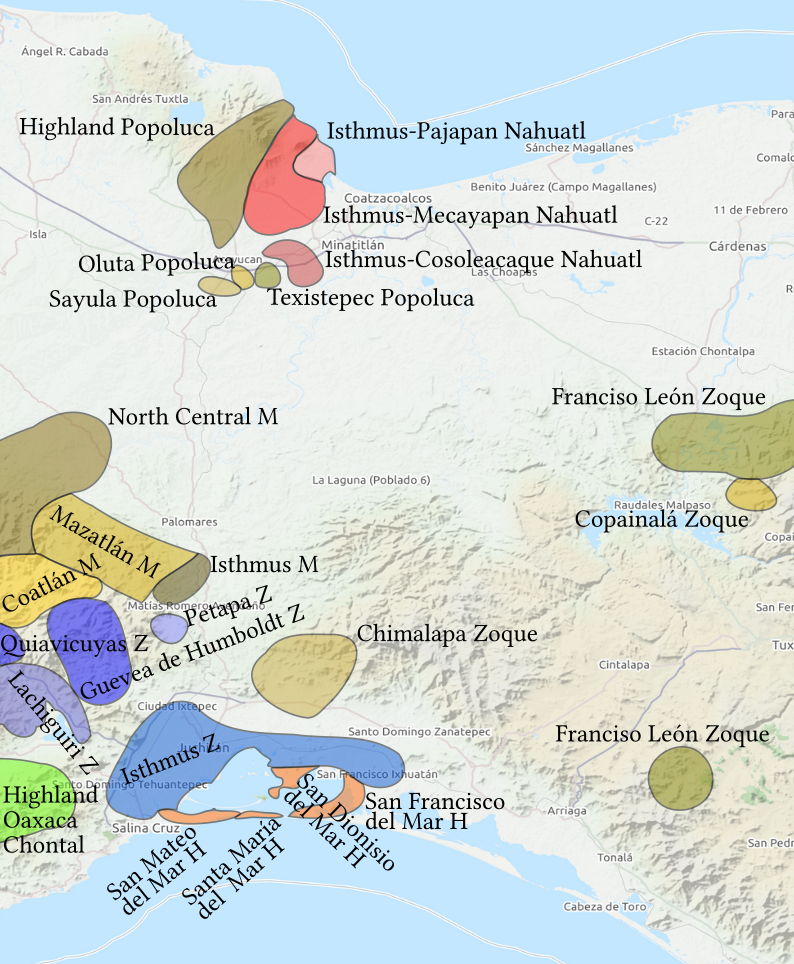
\includegraphics[height=.4\textheight]{figures/newmap.pdf}
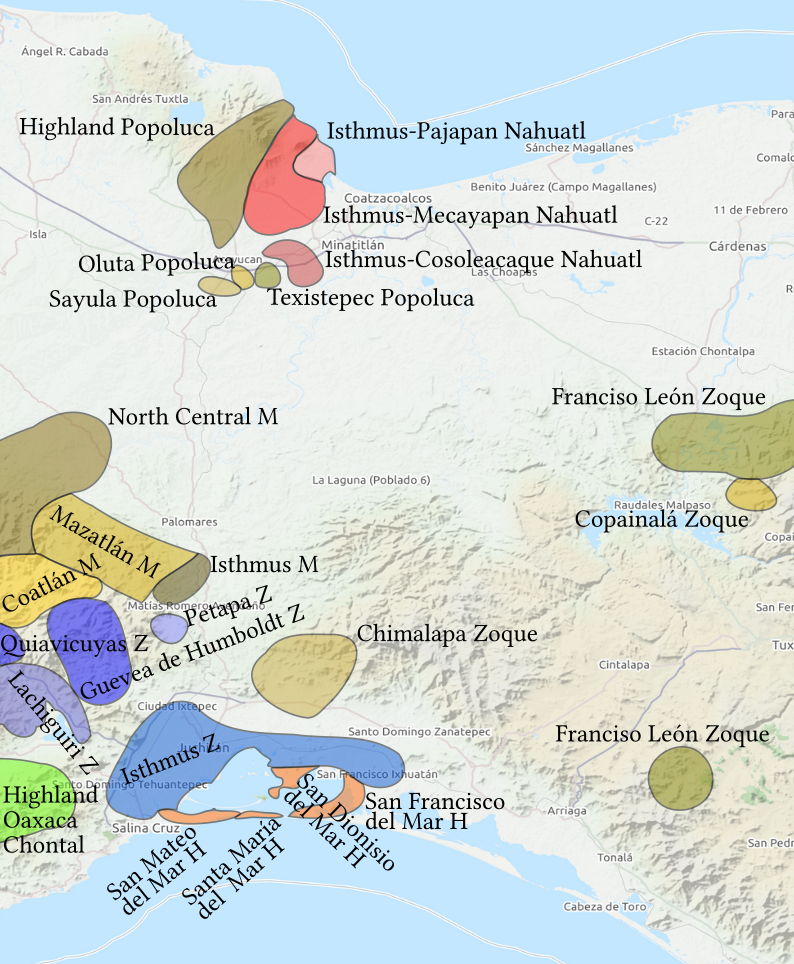
\includegraphics[height=.4\textheight]{figures/newmap.png}
\caption{{A linguistic map of the Isthmus of Tehuantepec (based on \citealt{lewis2016})}. Language families represented are
Nahuatl (red),
\ul{M}ixe-Zoquean (tan),
\ul{Z}apotec (blue),
Chontal (green),
\ul{H}uave (orange).
}
%\label{fig:chapterhandle:keytofigure}
\end{figure}


\largerpage[-1]
Still, for almost five centuries, \ili{Spanish} has served as the language of government, of the formal job market, and of the mainstream media and, increasingly with each generation, is replacing the indigenous language.\footnote{This is true for all or most of the indigenous languages across the country. The complex socio-political process that has led to this situation is the subject of \citet{heath1972}.}  Today, the impact of \ili{Spanish} on ZAI is even stronger than it has ever been, especially since the expansion of the public school system and instruction in \ili{Spanish} about 50 years ago. Although the percentage of ZAI-speaking residents older than 50 is quite high, the percentage of children that are growing up speaking the language is comparatively low, hovering around 50\% \citep{augsburger2004}. So, although stable \ili{Spanish}-ZAI bilingualism has been the norm for several centuries, in many areas the language shift from ZAI to \ili{Spanish} is now occurring very quickly and may even complete itself within the next generation \citep{augsburger2004}.

\isi{Juchitán} is distributed geographically into sections and, with the growing population, the city has extended beyond the original eight sections. In this growth, it is increasingly noticeable that the divisions between the sections mark patterns of language use such that these patterns roughly correlate with socio-economic differences.  Although the adult population is overwhelmingly bilingual throughout the city, certain sections of the city, like the \textit{s\'{e}ptima} and \textit{cheguigo} contain the majority of the ZAI-dominant speakers. These sections also contain higher concentrations of people engaged in traditional occupations, such as artisans and fishermen. In contrast, sections such as the \textit{primera},  \textit{segunda} and  \textit{tercera} are \ili{Spanish}-dominant. These sections are middle-class neighborhoods and contain a wider range of occupations.\footnote{See \citet{saynes2002}, \citet{augsburger2004}, and \citet[Chapter 1]{mccomsey2015} for a more detailed description of the socio-linguistic make-up of the city with respect to its sections. In towns such as Xadani and San Blas, which border the main urban areas of \isi{Juchitán} and Tehuantepec, respectively, and supply them with much of the manual labor, the percentages of residents older than 50 and of children between five and nine years who speak (or, at least, report speaking) ZAI are significantly higher. In other Isthmus towns as well as in Tehuantepec, the governmental center of the Isthmus, these percentages are much lower. See also \citet{toledo2018}.} 

One significant outcome, then, of the increasing rate of shift of the younger generation in favor of \ili{Spanish} is that the range of use of ZAI is being gradually reduced to specific sections of the city as well as to certain social networks with specific socioeconomic characteristics. The reduction in the range of social situations and communicative contexts in which ZAI is employed will no doubt have a strong impact on the diversity of genres and styles in which it will come to be used in day-to-day life and, concomitantly, on the forms and functions of the spoken language itself.

%The configuration of the community in these ways and in an urban setting creates a community in which speakers are exposed to both ZAI and \ili{Spanish} in different ways. The resultant differences in proficiency, as well as in the social networks that emerge in each of the sections of the city, in turn favor different patterns of language use. 


\section{Previous work on the language}
\largerpage
The linguist Velma Pickett is responsible for a great majority of the early linguistic documentation and analysis of ZAI.  Beginning her work on ZAI in the 1950's, much of Pickett's work in those years culminated in her doctoral thesis entitled \textit{The grammatical hierarchy of Isthmus Zapotec} \citep{pickett1960}, which focused primarily on a syntactic analysis of the language from the perspective of tagmemic grammar developed by Kenneth Pike. Pickett continued her work on ZAI and, with the establishment of the orthographic conventions, created a dictionary \citep{pickett1979} and, with Cheryl Black and Vicente Marcial Cerqueda, developed a concise speaker grammar \citep{pickett1998}. The dictionary and grammar together give an accurate, though very general, picture of the major aspects of the ZAI lexicon, phonology, morphology and syntax. Following Pickett's work, in the 1980's Carol Mock published several very thorough articles on the lexical phonology of ZAI \citep{mock1983,mock1985a,mock1985b,mock1988}. At around the same time, Pickett co-authored an article with Stephen Marlett entitled ``The syllable structure and aspect morphology of Isthmus Zapotec'' \citep{marlett1987}, which offers a very good description of the ZAI syllable and the complex system of aspectual prefixes. 

To my knowledge, only one documentation project of ZAI has been undertaken since the work of Pickett. This was done as part of the Project for the Documentation of the Languages of Meso-America (PDLMA). This project is ongoing and is primarily dedicated to the building of a lexicon \citep{perezms}. Neither the documentation of \isi{prosody} at the phrase or discourse level nor the documentation of \isi{information structure} are part of that project. 

Therefore, no studies on narrative discourse or \isi{information structure} in ZAI have been published or even conducted. Moreover, studies on discourse are extremely lacking for the great majority of Zapotec languages as well. One significant exception to this is the work by Mark Sicoli (\citealt{sicoli2007,sicoli2010}) on the use of \isi{tone} and \isi{intonation} in Lachix\'{i}o Zapotec (an Eastern Zapotecan language). Other existing work on Zapotec discourse has been done by linguists affiliated with the Summer Institute of Linguistics (SIL)  \citep{persons1979,long1985,benton1987,benton1997,kreikebaum1987,riggs1987,ward1987,piper1995,heise2003,riggs2010}. These studies have primarily descriptive goals, they tend to \isi{focus} on folk and written narrative, and are concerned mostly with specific syntactic problems and analyses at the sentence or paragraph level. Virtually no attention is paid to the role of \isi{intonation} or to the major components of \isi{information structure}.

Because of these studies and because of the amount of knowledge already gained in the areas of phonology, morphology, lexicon, and syntax, the opportunity to document and analyze \isi{information structure} in ZAI is open. The present project looks to build on this wealth of previous work. The close study of ZAI offers a unique opportunity to explore the possible combinations of \isi{prosody}, morphology and \isi{verb-initial syntax} that may occur in the coding of \isi{information structure}. Establishing the correlations between these areas is best determined by the analysis of spontaneous discourse. At the same time, however, one of the most straightforward ways to determine the range of possible constructions is via elicitation since this methodology makes it possible to create unambiguous contexts which trigger clearly distinct \isi{topic} and \isi{focus} structures. In this study, I take both methodological approaches. The rationale for utilizing this combination of methodologies is discussed in the next section.


\section{Methods}

\largerpage[-1]
In collecting the corpus that is the basis for this study, I worked with bilingual ZAI-\ili{Spanish} language consultants in \isi{Juchitán} over a 17-month period to record, transcribe, annotate and translate spontaneous speech and collect elicited native speaker judgments of constructed examples. The description that follows of \isi{information structure} of the language fills a crucial gap in the empirical base of knowledge about ZAI as well as Zapotec languages more broadly, and contributes important data for more general theoretical questions about language structure and use.

\subsection{Corpus creation}

During the fieldwork stage, I recorded spontaneous speech and supplemented this with data from elicitation through traditional field methodologies. The collected recordings ensure that naturally-occurring speech forms have been documented while the elicitation sessions  ensure that these forms are considered with respect to a broader set of possible combinations of \isi{tone} types, \isi{intonation} patterns and constituent orders. In the end, the documentary corpus allows for a more complete understanding of the range of constructions that are available to ZAI speakers and how they are employed to respond to specific discourse motivations.

In this, the project adopts a ``discourse-centered approach" for documentation and description \citep{sherzer1987}. Focusing on naturally-occurring speech makes it possible to find and analyze words and structures that may not surface when sentences from the contact language are translated into the target language. 

There are several reasons for focusing this documentation project on spontaneous speech. First, in contrast to other types of spoken genres such as ritual speech or traditional folklore which often tend to be formulaic, spontaneous speech and dialogue have the advantage of being naturally-occurring while providing extensive information about \isi{information structure}. Second, it offers the possibility of simultaneously documenting popular oral histories. Third, spontaneous speech is cross-linguistically under-documented. Fourth, the long scholarly tradition and extensive analysis of conversation across disciplines in the social sciences and humanities offers a solid foundation upon which linguistic analyses can be carried out as well as a potentially fruitful avenue to pursue in the dissemination of the data. In the end, by focusing on spontaneous speech, this project underlines the importance of documenting a speech genre that is meaningfully embedded in the daily social lives of the speakers. 

Still, it is important to recognize that specific constructions, word or \isi{intonation} contours of interest might occur only very rarely in running speech, which makes it impractical to rely solely on free narrative and/or conversation for linguistic research of pre-determined phenomena. This is the point made by \citet{himmelmann2006}, specifically with respect to the documentation of \isi{prosody}, which a part of this project will be particularly concerned with. To this end, structured games and nonlinguistic triggers such as pictures and short video clips, were employed in elicitation sessions designed to document a range of intonational contours and constituent orders.

As noted above, Zapotecan languages are well known for being phonologically complex, containing complex interactions between \isi{tone}, stress, and voice quality modifications such as \isi{glottalization} and larygealization. The documentation of ZAI discourse represents a chance to document the interesting phonological and phonetic variations of the language in use and the annotation and analysis of prosodic phenomena form a central part of this project.\footnote{After all, not marking \isi{prosody} in transcription may result in ``making something perfectly determined in speech undetermined in transcription'' \citep[57]{scarano2009}.}  

%For this, the ToBI (Tone and Break Indices) transcription system, which has been usefully applied cross-linguistically, will be employed. Specific work within this framework that will provide background for the project are Pierrehumbert (1980), Pierrehumbert and Beckman (1988), Jun (2005) (and the articles therein) and Sicoli (2007).


\subsection{A discourse corpus}

The collection of material for the discourse corpus employed native speakers of ZAI as language consultants and used the following data collection methods: 1) audio and audiovisual recording of naturally occurring speech, and 2) transcription and analysis of the data. The main purpose was to begin a collection of recordings with samples of spontaneous speech, something not represented currently in any archives of the language. 

The language is undergoing shift, so it was important to responsibly archive the data for future researchers and community members. Because of the hot and humid climate and because the majority of recordings were done outdoors, I used a Zoom H4n recorder and a Sony ECM-MS 957 external microphone as well as lavalier microphones. Audio recordings were made at a sampling rate of 16 bit/44 Khz. Visual recordings were made using a digital video camcorder with the same external microphones. All recordings were digitized and converted into WAV, MPEG1 and MPEG2 files to conform to Open Language Archives Community (OLAC) standards. 

In-field processing of the data included the transcription, translation and annotation of the recordings with the help of native-speaker language consultants (but not the speakers themselves). The texts were represented and time-aligned to the primary data using ELAN software in a multi-tiered analysis: orthography using the Isthmus Zapotec conventions; a morpheme-by-morpheme tier with glosses in \ili{Spanish} and \ili{English} using transparent terminology; and free translations in both \ili{Spanish} and \ili{English}. All phonetic analysis was done using Praat. 

\largerpage
Metadata for each recording is provided based on the International Standards for Language Engineering Metadata Initiative (IMDI) so as to ensure that all the relevant metadata is systematically and transparently documented. The audio and video recordings have been archived at the Endangered Languages Archive Repository (ELAR) of the Endangered Languages Documentation Programme at the School of Oriental and African Studies of the University of London. They are accompanied by transcriptions of the data and metadata files with information for each recording, all done in XML format. 	

The benefits of utilizing these standard documentation practices are twofold: they facilitate the proper archiving of the materials and the wider use of the resources by other people, including the community itself and they also facilitate future analyses by allowing for searches across structured annotations.



\section{Organization of the study}

This chapter discusses the motivation and objectives of the project and presents background information on Isthmus Zapotec and the speech community that is the subject of the research. It briefly describes the Isthmus Zapotec speaking population and characterizes the language's endangered status along with the socio-historical and cultural factors that shape the current linguistic situation. It surveys the existing documentation for ZAI, showing how the documentation of discourse aims to fill an important gap in the current documentation of the language. The chapter concludes with a review of the methodology employed in the data collection and creation of the corpus.

The following chapter presents a grammatical sketch of ZAI. It addresses the most relevant typological characteristics of the language, including, the phonological system, the structural function of \isi{prosody}, and \isi{verb-initial syntax}, focusing specifically on the role of \isi{constituent order} in the expression of \isi{information structure} in ZAI and showing the pre-verbal position to be the locus for a variety of discourse functions. It concludes with a summary of the main research questions that guide the rest of the study.

The main objective of \chapref{paschapter} is to explore the relationship between, first, the form and distribution of nominals and, second, their function in discourse to introduce and track referents and to mark referents as more or less accessible.  This discussion is framed in terms of the combined lens of \isi{Preferred Argument Structure} and Accessibility theory. It then moves on to a discussion of the cognitive status of the various nominal forms available to ZAI speakers. \chapref{alternation} focuses specifically on the contrast between the overt \textsc{3sg} subject enclitic and a \isi{zero form}. It explores the distribution and alternation of the two \isi{third person} clitics in narrative and conversation and argues that an important factor governing the use of these forms is the relative thematic \isi{salience} of third-person referents.  

The goal of \chapref{focuschapter} is to analyze the \isi{focus} structures available in ZAI. It does so by presenting a survey of the main \isi{focus} marking constructions of \isi{sentence focus}, \isi{predicate focus}, and \isi{argument focus} \citep{lambrecht1994} in order to place ZAI \isi{information structure} within the \isi{typology of focus structure} proposed by \citet{vanvalin1999}. The chapter explores the extent to which ZAI may be considered a more or less "rigid" \isi{verb-initial language} with respect to the kinds of pragmatically-marked information that may appear in pre-verbal position. The chapter ends with the consideration of a parallel use of sequenced \isi{predicate focus} and \isi{argument focus} constructions in conversation. 

\chapref{topicchapter} extends the analysis and the observations made in previous chapters to provide an analysis of the main \isi{topic} marking strategies in ZAI, including presentational, \isi{topic-comment}, and identificational constructions. The chapter ends with a discussion of the particle \textsc{la} and its functions in conversation to mark pre-posed \isi{adverbial} clauses and left-detached contrastive topics and, more generally, to negotiate and secure common ground between interlocutors. 


The final chapter summarizes the main conclusions of the study and proposes avenues of further research.





